\section{Proposed Approach}
\label{SecApproach}

Our approach consists of two phases: Source Code Analysis and Relationship Analysis.
In the first phase, Source Code Analysis, we take as input two revisions of a system, $v_1$ and $v_2$, and build two models that represent their source code.
Both models have the form of a tree, in which each node corresponds to a code element (classes, functions, etc.).
In the second phase, Relationship Analysis, we compute a set $R$, which contains triples of the form $(n_1, n_2, t)$, where $n_1$ is a code element from revision $v_1$, $n_2$ is a code element from revision $v_2$ and $t$ is a relationship type.
Such relationships may denote a high-level refactoring operation (move, rename, extract, etc.) or an exact correspondence between the code elements.
For example, consider the diff between two revisions of a system depicted in Figure~\ref{FigDiff1}.
Among other changes, the class \codeinl{Calculator}, declared in revision~1, is renamed to \codeinl{FpCalculator} in revision~2. This corresponds to a relationship of the type \emph{Rename} between them.
In the next sections, we describe in details each phase of our approach.

\begin{figure*}[htb]
\centering
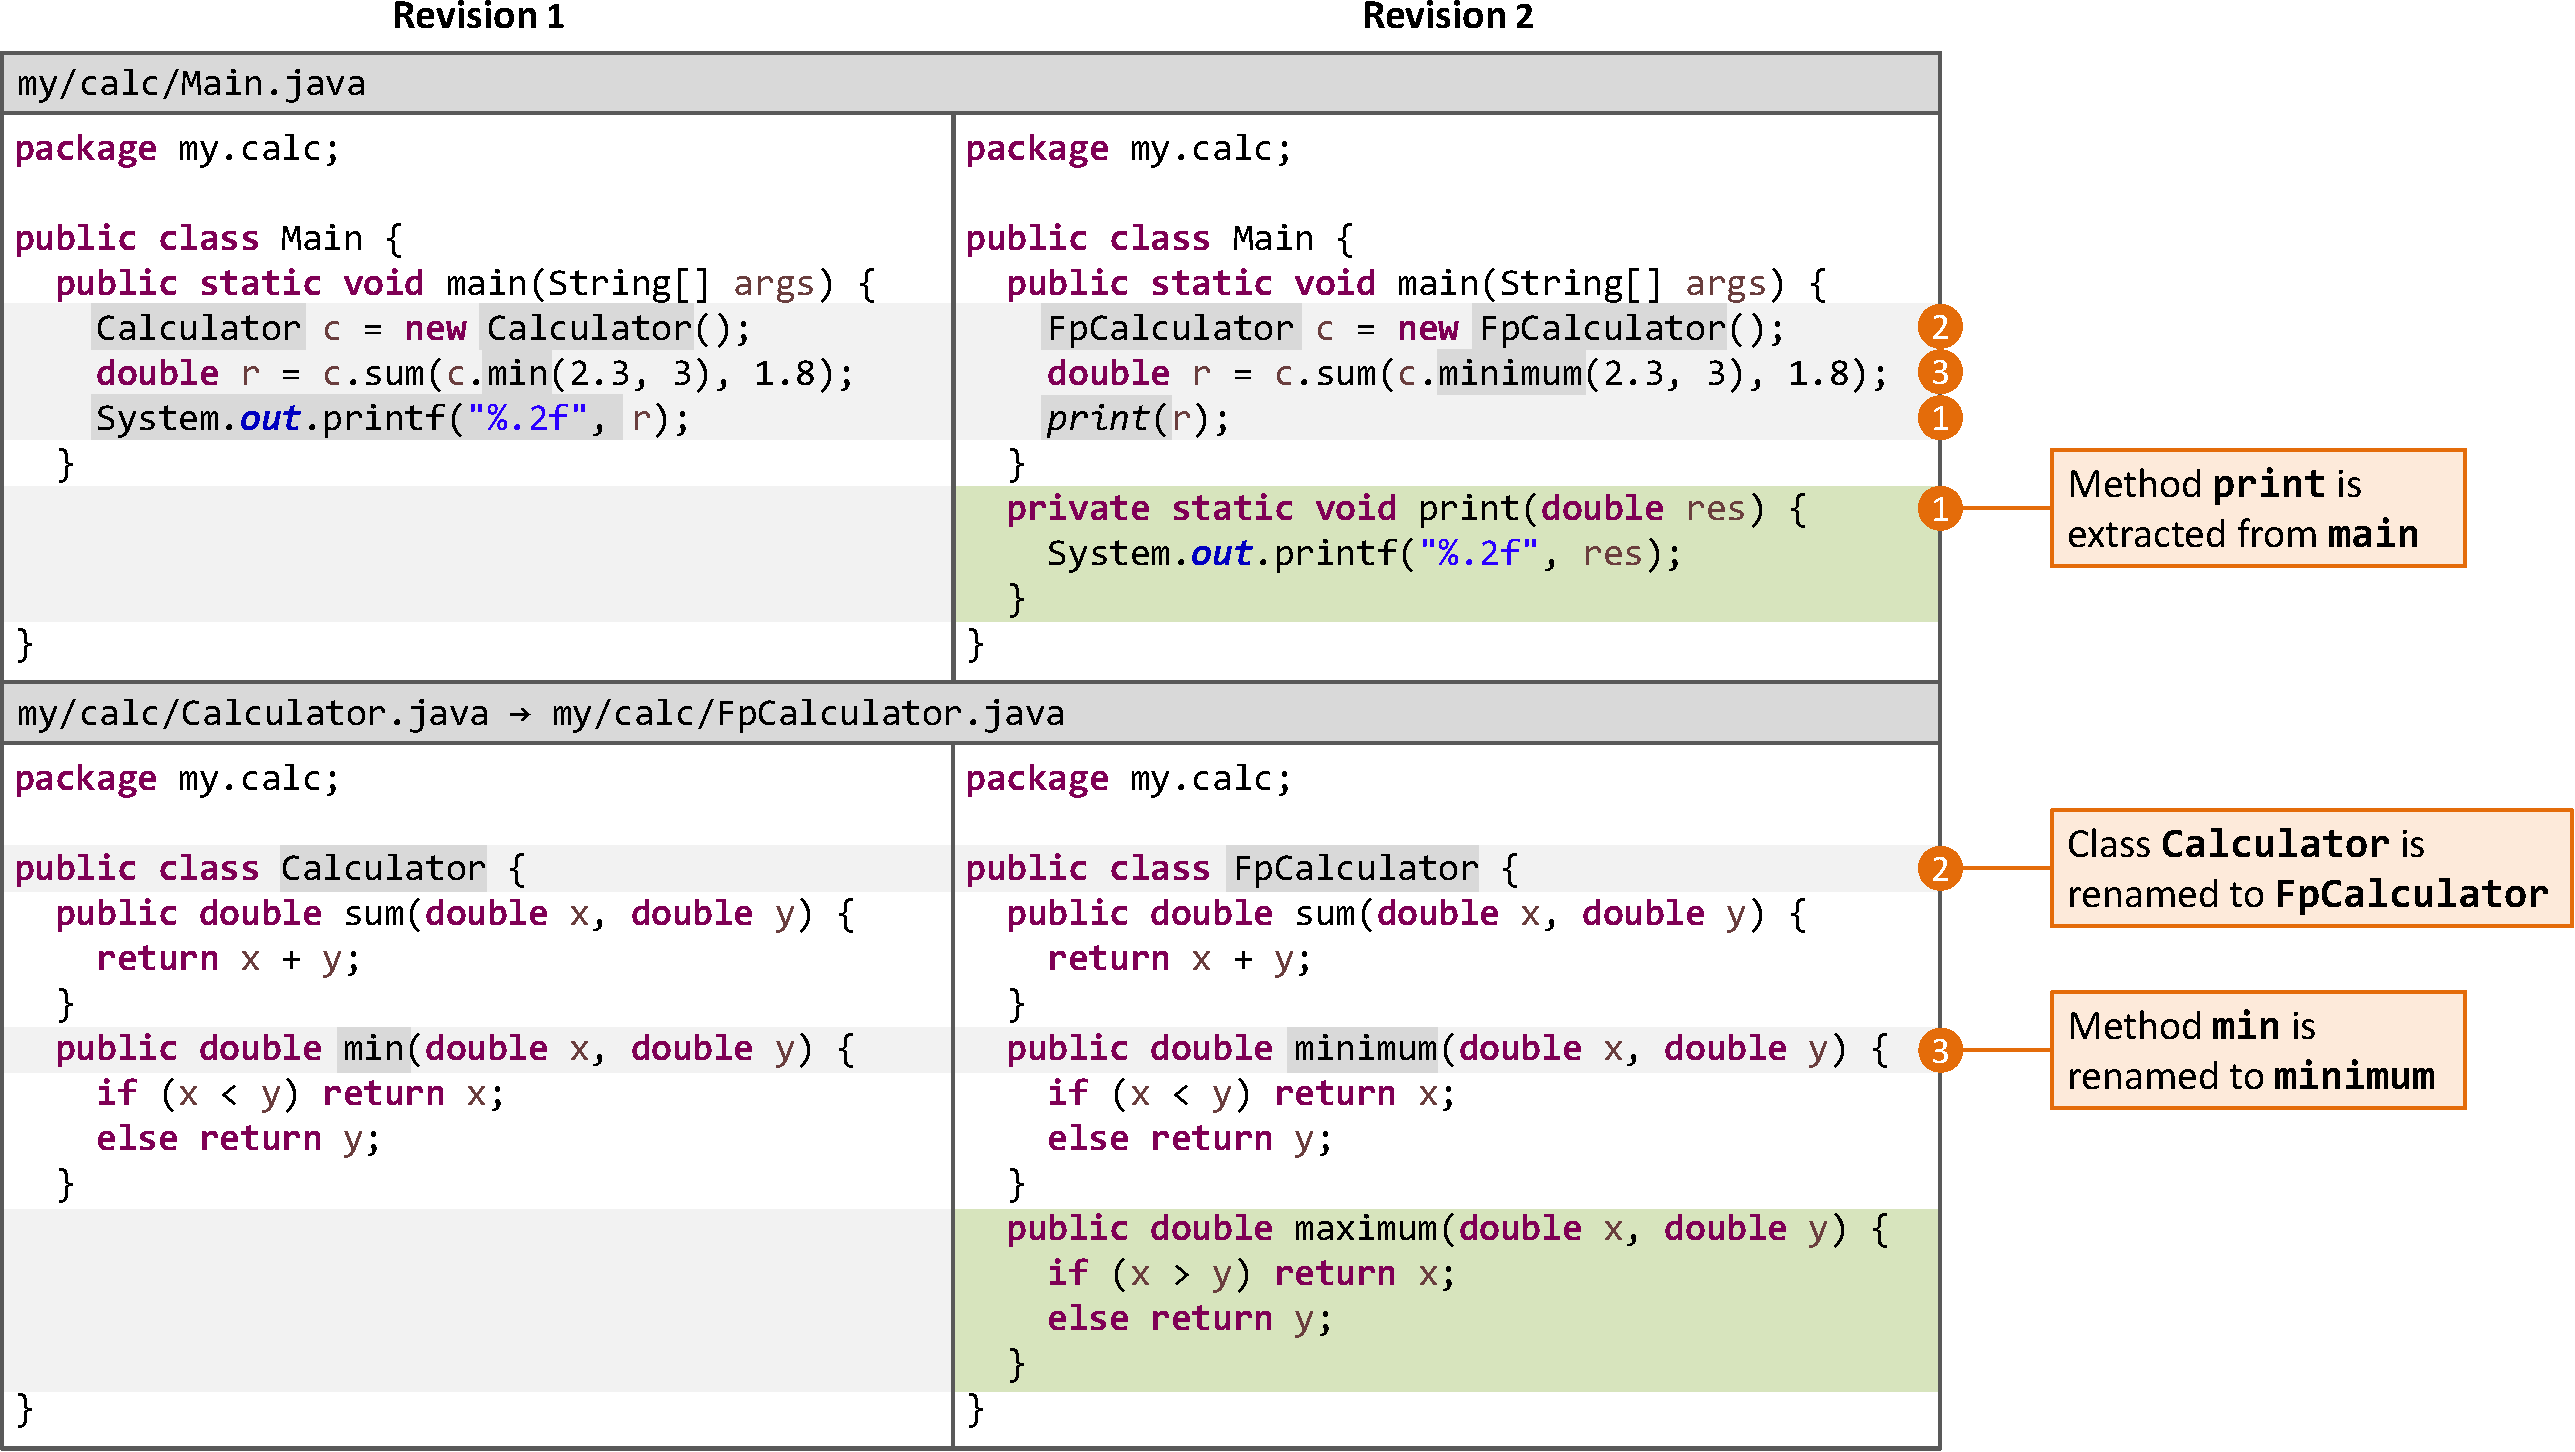
\includegraphics[width=0.9\textwidth]{img-diff1.pdf}
\caption{Illustrative diff between two revisions of a system annotated with refactoring operations}
\label{FigDiff1}
\end{figure*}


\subsection{Phase 1: Source Code Analysis}

The goal of this phase is to compute a language-independent model that represents the source code of the system, which we denote from now on as \emph{Code Structure Tree} (CST). The CST is a tree-like structure that resembles an \emph{Abstract Syntax Tree} (AST). However, in this representation we are only interested in coarse-grained code elements (e.g., classes and functions) that encompass a code region and may be referred by an identifier in other parts of the system.

To construct the CST, we need to parse the source code, generate the AST for the target programming language, and extract the necessary information.
Thus, the decision of which types of AST nodes become CST nodes depends on the programming language.
For example, in Java we represent classes, enums, interfaces, and methods as CST nodes.
In contrast, local variables are not represented.
Nevertheless, it is important to note that the granularity of the CST nodes determines the granularity of the relationships we are able to find, e.g., we can only find relationships between methods if we represent methods in the CST.
Table~\ref{TabCstNodes} lists the types of AST nodes that are represented in the CST for each programming language supported by the current implementation of our approach.

\begin{table}[htbp]
\renewcommand{\arraystretch}{1.2}
\caption{AST nodes that are represented in CSTs}
\label{TabCstNodes}
\centering
\begin{tabular}{@{}ll@{}}
\toprule
Language & Node types \\
\midrule
Java & class, enum, interface, and method \\
C & file and function \\
JavaScript & file, class, and function \\
\bottomrule
\end{tabular}
\end{table}

\begin{figure}[htb]
\centering
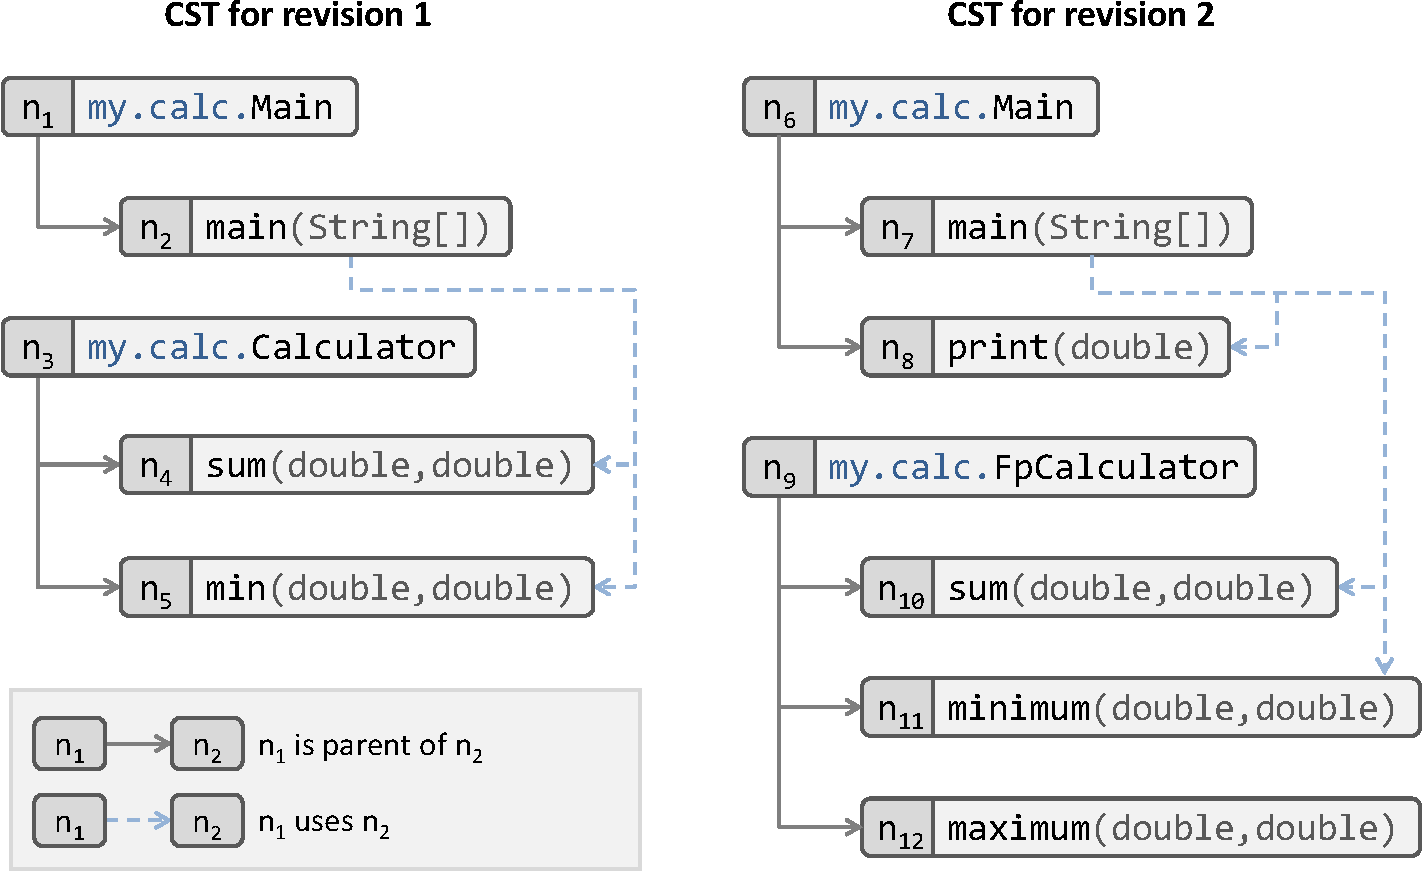
\includegraphics[width=1.0\linewidth]{img-cstDiff1.pdf}
\caption{CST of both revisions of the example system from Figure~\ref{FigDiff1}}
\label{FigJavaToCst}
\end{figure}

Figure~\ref{FigJavaToCst} exemplifies the transformation of the example system from Figure~\ref{FigDiff1} into a corresponding CST.
In revision~1, the class \codeinl{Main} is declared with a single method \codeinl{main} and the class \codeinl{Calculator} contains two methods: \codeinl{sum} and \codeinl{min}.
Note that these classes and methods become nodes in the CST for revision~1, preserving the same nesting structure of the source code. Analogously, the figure also depicts the CST for revision 2, which contains seven nodes in total (two classes and five methods).

Besides the representation of the code elements, the CST also embeds a simplified call graph and  a type hierarchy graph of the nodes within the CST, that is, there are edges to represent whether a certain node $n_1$ calls $n_2$, or whether $n_1$ is a subtype of $n_2$. The first information is necessary to find \emph{Extract} and \emph{Inline} relationships between code elements, while the second is used to find inheritance-related relationships, such as \emph{Pull Up} and \emph{Push Down}.

Moreover, along with each node of the CST, we store the following information:
\begin{description}
    \item[Identifier] \hfill \\
    An identifier of the code element in its declared scope. 
    The identifier is usually the name of the code element, but it may also contain additional information to avoid ambiguities.
    For example, the identifier of the class \codeinl{Calculator} from Figure~\ref{FigJavaToCst} is simply its name, but the identifier of the method \codeinl{sum} is \codeinl{sum(double,double)},  because there could be an overloaded method with a different signature.
    
    \item[Namespace] \hfill \\
    An optional prefix that, along with the identifier, globally identifies the code element. 
    This information only applies to top-level nodes and corresponds to the package or folder that the element is contained. For example, the namespace of the class \codeinl{Calculator} from Figure~\ref{FigJavaToCst} is \codeinl{my.calc.}.
    
    \item[Node type] \hfill \\
    A string that identifies the node type in the target language (class, function, method, etc.).
    
    \item[Parameters list]  \hfill \\
    An optional list of the name of the parameters, in the case the node corresponds to a method or function.
    
    \item[Tokenized source code]  \hfill \\
    The source code of the element in the form of a list of tokens.
    Here, we include all tokens in the code region that encompasses the complete declaration of the code element, including its name/signature.
    This information is necessary to compute the similarity between code elements, as explained in Section~\ref{SecCodeSim}.
    
    
    \item[Tokenized source code of the body]  \hfill \\
    The source code of the body of the code element in the form of a list of tokens.
    Here we include only the tokens within the body of the code element, but not its name/signature.
    This information is also necessary to compute the similarity between code elements in the special cases of \textit{Extract} and \textit{Inline} relationships, as explained in Section~\ref{SecSimX}.
    It is worth noting that this information is optional, as not every node has a body (e.g., abstract methods).
    
\end{description}

It is worth noting that we generate the CST only for source files that have been added, removed, or modified between revisions. 
Such information can be efficiently obtained from version control systems, without the need to analyze the content of all files within the repository.
This way, we avoid a costly operation that might compromise the scalability of our approach, as large repositories contain thousands of source files, but only a small fraction of them change between revisions.

Although the construction of the CST is a language-specific process, from this point on, the approach is language-independent and relies only on information encoded in CSTs.
This way, one is able to extend our approach to work with different programming languages only by implementing the \emph{Source Code Analysis} module.
To demonstrate this capability, we provide implementations for three programming languages: Java, C, and JavaScript.


\subsection{Phase 2: Relationship Analysis}

This phase takes as input the CST's of revisions $v_1$ and $v_2$ and outputs the set of relationships $R$. Let $N_1$ and $N_2$ be the sets of code elements from the CST's of $v_1$ and $v_2$ respectively. Each relationship $r \in R$ is a triple $(n_1, n_2, t)$, where $n_1 \in N_1$, $n_2 \in N_2$, and $t$ is a relationship type. The types of relationships are listed in the first column of Table~\ref{TabRelationshipTypes}, and can be subdivided into two groups:
\begin{itemize}
\item \textbf{Matching relationships}, which indicate that the node $n_1$ corresponds to $n_2$ in the subsequent revision.
The possible matching relationships are \textit{Same}, \textit{Convert Type}, \textit{Pull Up}, \textit{Push Down}, \textit{Change Signature}, \textit{Move}, \textit{Rename}, and \textit{Move and Rename}.
We say that a node $n_1$ matches with $n_2$ if exists a relationship $(n_1, n_2, t) \in R$ such that $t$ is a matching relationship.

\item \textbf{Non-matching relationships}, which indicate that either node $n_1$ is decomposed to create $n_2$, or node $n_1$ is incorporated into $n_2$.
There are four non-matching relationships: \textit{Extract Supertype}, \textit{Extract}, \textit{Extract and Move}, and \textit{Inline}.
\end{itemize}


\subsubsection{General algorithm to find relationships}

\begin{figure}[htbp]
\small
%\fontsize{9.5}{10.5}\selectfont
\begin{algorithmic}[1]
\Procedure{FindRelationships}{$t_1,t_2$}
\State $R \gets \emptyset$
\State $M \gets \emptyset$
\State $\textsc{findMatchingsById}(t_1,t_2)$
\State $\textsc{findMatchingsBySim}$
\State $\textsc{findMatchingsByChildr}$
\State $\textsc{resolveMatchings}$
\State $\textsc{findNonMatchingRel}$
\State \Return $R$
\\
\Procedure{findMatchingsById}{$p_1,p_2$}
\ForEach{$(n_1, n_2) \in \rdchildren(p_1) \times \rdchildren(p_2)$}
  \If {$\rdsig(n_1) = \rdsig(n_2) \land \rdns(n_1) = \rdns(n_2)$}
    \State $\textsc{addMatch}(n_1, n_2)$
  \EndIf
\EndFor
\EndProcedure
\\
\Procedure{findMatchingsBySim}{}
\ForEach{$(n_1, n_2) \in \rdsortbysim(N^- \times N^+)$}
  \If {$\mathit{findMatchRel}(n_1, n_2) \neq \emptyset$}
    \State $\textsc{addMatch}(n_1, n_2)$
  \EndIf  
\EndFor
\EndProcedure
\\
\Procedure{findMatchingsByChildr}{}
\ForEach{$(n_1, n_2) \in \rdsortbysim(N^- \times N^+)$}
  \If {$\mathit{matchingChildr}(n_1, n_2) > 1\,\land \newline
    \hspace*{5.5em} \rdnsim(n_1, n_2) > 0.5$}
    \State $\textsc{addMatch}(n_1, n_2)$
  \EndIf
\EndFor
\EndProcedure
\\
\Procedure{resolveMatchings}{}
\ForEach{$(n_1, n_2) \in M$}
  \State $R \gets R \cup \mathit{findMatchRel}(n_1, n_2)$
\EndFor
\EndProcedure
\\
\Procedure{findNonMatchingRel}{}
\ForEach{$(n_1, n_2) \in M_1 \times N^+$}
  \State $R \gets R \cup \mathit{findExtractSupertype}(n_1, n_2)$
  \State $R \gets R \cup \mathit{findExtract}(n_1, n_2)$
  \State $R \gets R \cup \mathit{findExtractMove}(n_1, n_2)$
\EndFor
\ForEach{$(n_1, n_2) \in N^- \times M_2$}
  \State $R \gets R \cup \mathit{findInline}(n_1, n_2)$
\EndFor
\EndProcedure
\\
\Procedure{addMatch}{$n_1, n_2$}
\If {$n_1 \in N^- \land n_2 \in N^+$}
  \State $M \gets M \cup \{(n_1, n_2)\}$
  \State $\textsc{findMatchingsById}(n_1,n_2)$
\EndIf
\EndProcedure
\\
\EndProcedure
\end{algorithmic}
%\vspace{1em}
%{
%\footnotesize
%\renewcommand{\arraystretch}{1.3}
%\begin{tabular}{@{}ll@{}}
%\midrule
%\multicolumn{2}{c}{\textbf{Definitions}}\\
%$\rdchildren(n)$ & set of children of $n$ in the CST\\
%$\rdsortbysim(S)$ & elements of $S$ sorted by $\rdsim$ function descending\\
%\midrule
%\end{tabular}
%}
\caption{Algorithm to find relationships}
\label{AlgoGeneral}
\end{figure}






Our approach employs the algorithm described in Figure~\ref{AlgoGeneral} to find the relationships (i.e., to compute the set $R$).
The procedure \textsc{FindRelationships} has two parameters, $t_1$ and $t_2$, which are the root nodes of the CST's of both revisions.
Initially, we define $R \gets \emptyset$ as the set of relationships found so far (line~2).
Additionally, we also define $M \gets \emptyset$ as the set of pairs of matching nodes found so far (line~3).
Then, we execute four subroutines:
\begin{enumerate}

\item In \textsc{findMatchingsById}, we recursively look for matching nodes that have the same identifier and parent, i.e., we assume that code elements with the same identifier and parent are the same. In the case of top-level nodes, which do not have parents, their namespace should be the same.
Such assumption allows us to match many code elements at this step, reducing the number of possibilities that need to be checked in the next steps.
The procedure consists of a loop that pairs the children of the nodes received as arguments and calls the procedure \textsc{addMatch} whenever a matching is found (line~13).
On its turn, \textsc{addMatch} (lines 46-51) adds a pair of matching nodes to $M$ and calls \textsc{findMatchingsById} again to look for matchings on their children, completing the recursion.
The matching pairs found in this step will be resolved to \textit{Same} and \textit{Convert type} relationships later (see step~4).

\item In \textsc{findMatchingsBySim}, we look for matching nodes based on code similarity.
The goal is to find \textit{Change Signature}, \textit{Pull Up}, \textit{Push Down}, \textit{Move}, \textit{Rename}, and \textit{Move and Rename} relationships.
%The procedure starts by computing the set $M'$, which contains unmatched pairs of nodes from $t_1$ and $t_2$.
The procedure iterates over the unmatched pairs of nodes sorted by similarity in descending order.
We use the notation $N^-$ to denote the set of unmatched nodes from $t_1$ (presumably deleted) and $N^+$ to denote the set of unmatched nodes from $t_2$ (presumably added).
For each pair $(n_1, n_2)$, the procedure checks if it meets the conditions (specified in the second column of Table~\ref{TabRelationshipTypes}) for any matching relationship by calling $\mathit{findMatchRel}(n_1, n_2)$.
%Then, it repeatedly takes a pair $(n_1, n_2)$ from $M'$, sorting by the $\rdrank$ function, and checks if it meets the conditions (specified in the second column of Table~\ref{TabRelationshipTypes}) for any matching relationship by calling $\mathit{findMatchRel}(n_1, n_2)$.
This function returns a singleton containing a matching relationship or an empty set if none of the conditions are met.
Last, the \textsc{addMatch} subroutine is called in the case of a matching (line~24).
The conditions to find those relationships and the $\rdsortbysim$ function rely on a code similarity metric, which is described in details in Section~\ref{SecCodeSim}.

\item In \textsc{findMatchingsByChildr}, we look for matching nodes based on matchings of their children and name similarity. 
Once again, the procedure iterates over the unmatched pairs of nodes sorted by similarity in descending order.
For each pair $(n_1, n_2)$, if $n_1$ has more than one children that match with $n_2$'s children and their names are similar, then we consider it a match. The $\rdnsim$ function, used to compute the similarity between names, is described in details in Section~\ref{SecNameSim}.
This heuristic is intended to cover the cases when a code element (e.g., a class) is moved (and/or renamed) and it is also subjected to many additions or removals of its members, so that its similarity with its matching pair is not enough to yield a match in the previous step.
Failing to detect that a class has been moved (or renamed) may yield several incorrect \textit{Move} relationships between its members before and after the change.


\item In \textsc{resolveMatchings}, we add the relationships corresponding to the matching pairs found at steps~1, 2, and 3 to $R$.
The procedure iterates over the elements of $M$ and calls $\mathit{findMatchRel}$ to find which relationship type holds between $n_1$ and $n_2$ (according to the conditions defined in Table~\ref{TabRelationshipTypes}).
By the end of this step, $R$ contains all matching relationships found.
The rationale for postponing the resolution of the relationship type is discussed in Section~\ref{SecDependentConflictingRel}.

\item In \textsc{findNonMatchingRel}, we look for non-matching relationships.
First, we iterate over the pairs of matched/unmatched nodes, i.e., $M_1 \times N^+$, to look for \textit{Extract Supertype}, \textit{Extract} and \textit{Extract and Move} relationships.
Similarly, we also iterate over the pairs of unmatched/matched nodes ($N^- \times M_2$) to search for \textit{Inline} relationships.
The functions $findExtractSupertype$, $findExtract$, $findExtractMove$, and $findInline$ check the  preconditions for the corresponding relationship types, according to Table~\ref{TabRelationshipTypes}.
After this last step, $R$ contains all matching and non-matching relationships between CST nodes of both revisions.
\end{enumerate}


\begin{table*}[htbp]
\renewcommand{\arraystretch}{1.3}
\caption{Definitions used in the Algorithm from Figure~\ref{AlgoGeneral} and in the conditions from Table~\ref{TabRelationshipTypes}}
\label{TabDefinitions}
\centering
\begin{tabular}{@{}lll@{}}
\toprule
%\multicolumn{3}{c}{\textbf{Definitions}}\\
\begin{tabular}{@{}ll@{}}
$M_1$ & the set of nodes from $N_1$ that matches with a node from $N_2$\\
$M_2$ & the set of nodes from $N_2$ that matches with a node from $N_1$\\
$N^-$ & the set of unmatched nodes from $N_1$ ($N_1 \setminus M_1$)\\
$N^+$ & the set of unmatched nodes from $N_2$ ($N_2 \setminus M_2$)\\
$n'$ & the code element that matches with $n$ in the other revision\\
$\rdparent(n)$ & parent of a node $n$ (it may be a namespace or a CST node)\\
$\rdns(n)$ & namespace of the code element $n$\\
$\rdchildren(n)$ & set of children of $n$ in the CST\\
\end{tabular}
& &
\begin{tabular}{@{}ll@{}}
$\rdname(n)$ & simple name of the code element $n$\\
$\rdsig(n)$ & identifier of the code element $n$\\
$\rdtype(n)$ & node type of the code element $n$\\
$\rdsub(n_1, n_2)$ & $n_1$ is subtype of $n_2$\\
$\rduses(n_1, n_2)$ & $n_1$ uses $n_2$\\
$\rdsim(n_1, n_2)$ & code similarity between $n_1$ and $n_2$\\
$\rdnsim(n_1, n_2)$ & name similarity between $n_1$ and $n_2$\\
$\rdsimx(n_1, n_2)$ & extract similarity between $n_1$ and $n_2$\\
$\rdsortbysim(S)$ & elements of $S$ sorted by $\rdsim$ descending\\
\end{tabular}
\\
\bottomrule
\end{tabular}

\end{table*}



\begin{table*}[htbp]
\renewcommand{\arraystretch}{1.3}
\caption{Relationship types and the conditions to find them}
\label{TabRelationshipTypes}
\centering
\begin{tabular}{@{}lll@{}}
\toprule
Relationship type & \multicolumn{2}{l}{Conditions} \\
\midrule
& \multicolumn{2}{l}{$(n_1, n_2) \in N^- \times N^+$, such that:}\\
Same & & $\rdtype(n_1) = \rdtype(n_2) \land \rdsig(n_1) = \rdsig(n_2) \land \rdparent(n_1)' = \rdparent(n_2)$ \\
Convert Type & & $\rdtype(n_1) \neq \rdtype(n_2) \land \rdsig(n_1) = \rdsig(n_2) \land \rdparent(n_1)' = \rdparent(n_2)$ \\
Pull Up & & $\rdtype(n_1) = \rdtype(n_2) \land \rdsig(n_1) = \rdsig(n_2) \land \rdsub(\rdparent(n_1)', \rdparent(n_2))$ \\
Push Down & & $\rdtype(n_1) = \rdtype(n_2) \land \rdsig(n_1) = \rdsig(n_2) \land \rdsub(\rdparent(n_2), \rdparent(n_1)')$ \\
Change Signature & & $\rdtype(n_1) = \rdtype(n_2) \land \rdsig(n_1) \neq \rdsig(n_2) \land \rdname(n_1) = \rdname(n_2) \land \rdparent(n_1)' = \rdparent(n_2) \land \rdsim(n_1, n_2) > 0.5$ \\
Move & & $\rdtype(n_1) = \rdtype(n_2) \land \rdname(n_1) = \rdname(n_2) \land \rdparent(n_1)' \neq \rdparent(n_2) \land \rdsim(n_1, n_2) > 0.5$ \\
Rename & & $\rdtype(n_1) = \rdtype(n_2) \land \rdname(n_1) \neq \rdname(n_2) \land \rdparent(n_1)' = \rdparent(n_2) \land \rdsim(n_1, n_2) > 0.5$ \\
Move and Rename & & $\rdtype(n_1) = \rdtype(n_2) \land \rdname(n_1) \neq \rdname(n_2) \land \rdparent(n_1)' \neq \rdparent(n_2) \land \rdsim(n_1, n_2) > 0.5$ \\
\addlinespace
& \multicolumn{2}{l}{$(n_1, n_2) \in M_1 \times N^+$, such that:}\\
Extract Supertype & & $\exists (n_3, n_4, \mathit{PullUp}) \in R\, (n_1 = \rdparent(n_3) \land n_2 = \rdparent(n_4))$ \\
Extract & & $\rduses(n_1', n_2) \land \rdparent(n_1)' = \rdparent(n_2) \land \rdsimx(n_2, n_1) > 0.5$ \\
Extract and Move & & $\rduses(n_1', n_2) \land \rdparent(n_1)' \neq \rdparent(n_2) \land \rdsimx(n_2, n_1) > 0.5$ \\
\addlinespace
& \multicolumn{2}{l}{$(n_1, n_2) \in N^- \times M_2$, such that:}\\
Inline & & $\rduses(n_1, n_2') \land \rdsimx(n_1, n_2) > 0.5$ \\
\bottomrule
\end{tabular}
\end{table*}







Figure~\ref{FigRelationships1} shows the relationships we find after running RefDiff in the example from Figure~\ref{FigDiff1}.
Each relationship is represented by an edge connecting nodes from the left and right CSTs.
There are three relationships of the type \textit{Same}, involving the code elements whose identifiers do not change: the class \codeinl{Main} and the methods \codeinl{main} and \codeinl{sum}.
Two of the relationships are of type \textit{Rename}, indicating that the class \codeinl{Calculator} is renamed to \codeinl{FpCalculator}, and the method \codeinl{min} is renamed to \codeinl{minimum}.
Moreover, there is an \textit{Extract} relationship indicating that the method \codeinl{print} is extracted from \codeinl{main}.
Finally, we can also note that two nodes, $n_8$ and $n_{12}$, are not involved in matching relationships. Thus, we classify them as added code elements.
In this example, as every node on the left side is matched, there are no deleted code elements.


\begin{figure}[htbp]
\centering
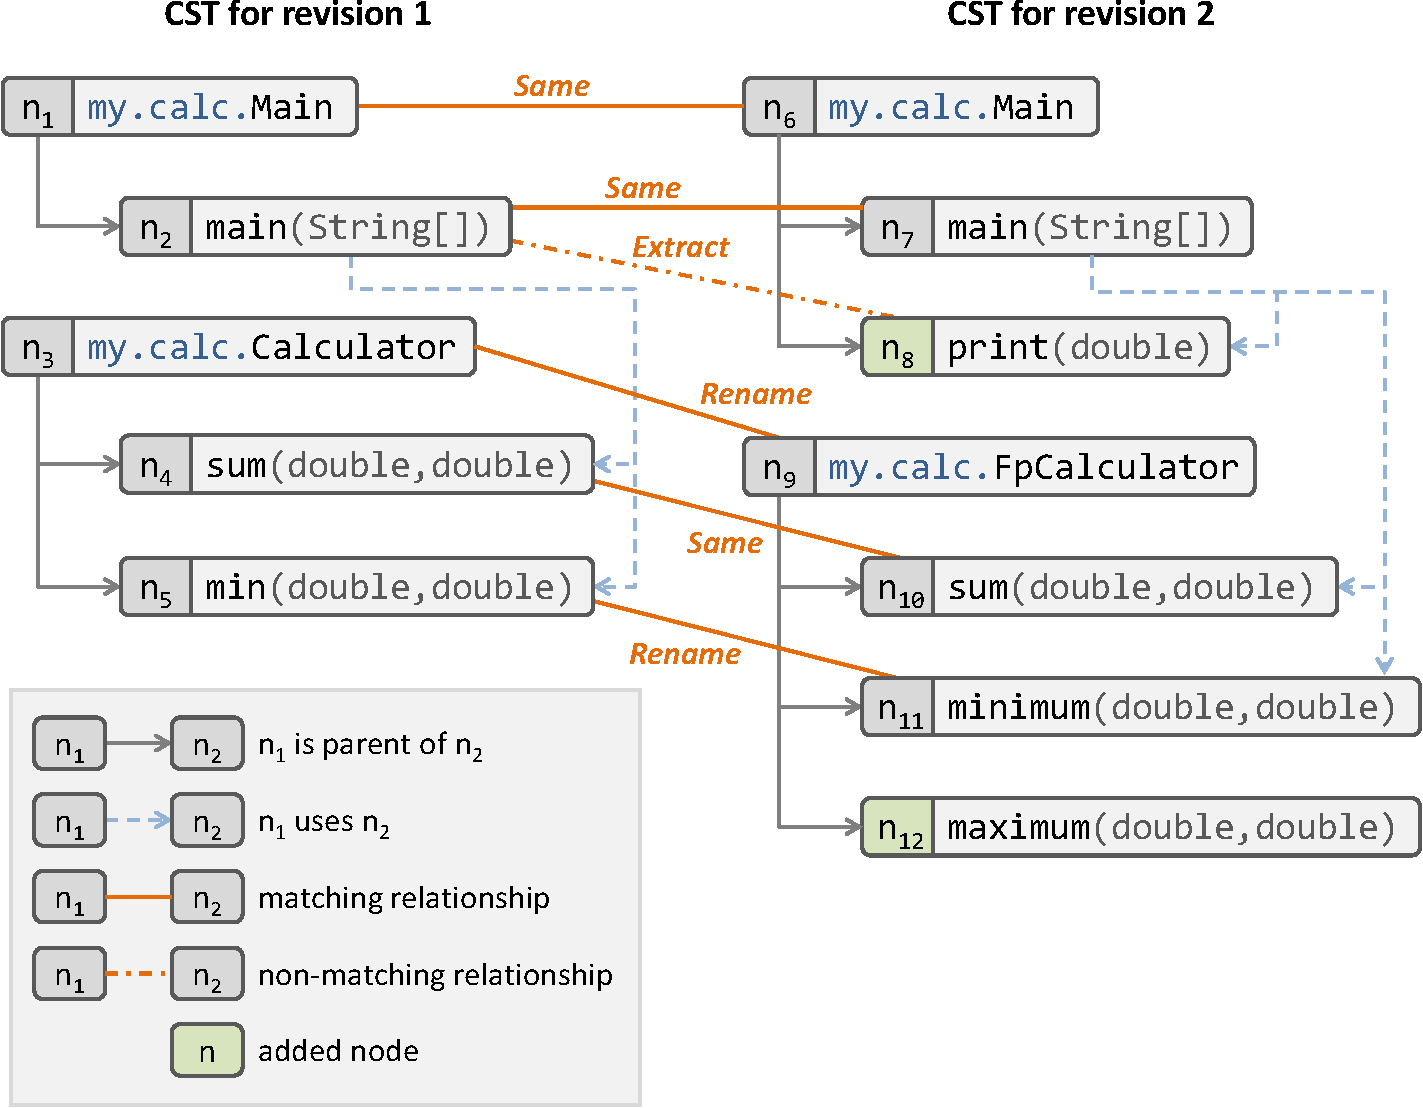
\includegraphics[width=1.0\linewidth]{img-relationshipDiff1.pdf}
\caption{Relationships found in the example from Figure~\ref{FigDiff1}}
\label{FigRelationships1}
\end{figure}


\subsubsection{Dependent and conflicting relationships}
\label{SecDependentConflictingRel}

In some cases, correctly finding a relationship depends on finding a prior relationship.
For example, consider the relationship $(n_5, n_{11}, Rename)$ in Figure~\ref{FigRelationships1} (method \codeinl{min} renamed to \codeinl{minimum}).
The conditions for this relationship includes the clause $\rdparent(n_5)' = \rdparent(n_{11})$, which means that the matching node of the parent of $n_5$ should be equal to the parent of $n_{11}$ (see Table~\ref{TabRelationshipTypes}, \textit{Rename} row).
This clause only yields true after the matching pair $(n_3, n_9)$ is added to $M$, i.e., after we find out that \codeinl{Calculator} is renamed to \codeinl{FpCalculator}.
In fact, if we call $\mathit{findMatchRel}(n_5, n_{11})$ before $M$ contains $(n_3, n_9)$, we would incorrectly classify it as a \textit{Move and Rename} relationship.
To address this issue, we only resolve the actual relationship types in steps~4 and~5, after all matching pairs are found (note that in steps~1, 2, and 3 we record the matching pairs in $M$, purposely ignoring the type of relationship).
%Moreover, non-matching relationships, which also depends on the matchings found, are analyzed in the last step. 


\begin{figure*}[htb]
\renewcommand{\arraystretch}{1.3}
\centering
\footnotesize
\begin{tabular}{@{}llll@{}}
\begin{tabular}{p{6.5cm}}
\multicolumn{1}{c}{\textbf{Source code of a class}} \\
\begin{lstlisting}
public class Calculator {

  public int sum(int x, int y) {
    return x + y;
  }

  public int min(int x, int y) {
    if (x < y) return x;
    else return y;
  }

  public double power(int b, int e) {
    return Math.pow(b, e);
  }
}
\end{lstlisting}\\

\end{tabular}
& {\Large $\Rightarrow$} &
\begin{tabular}{|l|r|r|r|}
\multicolumn{4}{c}{\textbf{Multiset of tokens for each method}} \\
\hline
Token $t$ & $m_{\mathtt{sum}}(t)$ & $m_{\mathtt{min}}(t)$ & $m_{\mathtt{power}}(t)$\\
\hline
\codeinl{return} & 1 & 2 & 1 \\
\codeinl{x}      & 1 & 2 & 0 \\
\codeinl{+}      & 1 & 0 & 0 \\
\codeinl{y}      & 1 & 2 & 0 \\
\codeinl{;}      & 1 & 2 & 1 \\
\codeinl{if}     & 0 & 1 & 0 \\
\codeinl{(}      & 0 & 1 & 1 \\
\codeinl{<}      & 0 & 1 & 0 \\
\codeinl{)}      & 0 & 1 & 1 \\
\codeinl{else}   & 0 & 1 & 0 \\
\codeinl{Math}   & 0 & 0 & 1 \\
\codeinl{.}      & 0 & 0 & 1 \\
\codeinl{pow}    & 0 & 0 & 1 \\
\codeinl{b}      & 0 & 0 & 1 \\
\codeinl{,}      & 0 & 0 & 1 \\
\codeinl{e}      & 0 & 0 & 1 \\
\hline
\end{tabular} &
\begin{tabular}{|r|}
\multicolumn{1}{c}{} \\
\hline
$n_t$\\
\hline
3 \\
2 \\
1 \\
2 \\
3 \\
1 \\
2 \\
1 \\
2 \\
1 \\
1 \\
1 \\
1 \\
1 \\
1 \\
1 \\
\hline
\end{tabular}
\end{tabular}
\caption{Transformation of the body of methods into a multiset of tokens}
\label{FigSourceCodeTransformation}
\end{figure*}



Another issue which we may face when looking for relationships are conflicts, i.e., two or more matching relationships hold for the same code element (according to conditions from Table~\ref{TabRelationshipTypes}).
For instance, in the example from Figure~\ref{FigRelationships1}, the conditions for \textit{Rename} yield true for the pair of methods \codeinl{min} and \codeinl{minimum} because their source code are similar and their parents match.
However, this is also the case for the pair of methods \codeinl{min} and \codeinl{maximum}, whose bodies are also similar.
We cannot match the same node twice, thus, we must decide upon which relationship we will accept and discard the other one.
This issue is addressed in procedures \textsc{findMatchingsBySim} and \textsc{findMatchingsByChildr} by using the $\rdsortbysim$ function to sort the potential matching pairs, enforcing that we take first the most likely matches.
The $\rdsortbysim$ function relies on a similarity metric, which we discuss in details in Section~\ref{SecCodeSim}.
After a matching pair $(n_1, n_2)$ is added to $M$, no more matchings involving $n_1$ or $n_2$ are accepted, because \textsc{addMatch} procedure checks that $n_1 \in N^- \land n_2 \in N^+$ (line~47).







\subsection{Code Similarity}
\label{SecCodeSim}



A key element of our approach to find relationships, as previously mentioned, is computing the similarity between code elements (i.e., CST nodes).
The first step to compute this similarity is to represent their source code as a multiset (or bag) of tokens.
A multiset is a generalization of the concept of a set, but it allows multiple instances of the same element.
The multiplicity of an element is the number of occurrences of that element within the multiset.
This representation provides two advantages for our approach.
First, it makes the CST simpler and less coupled to the syntax of programming languages, because we do not need to represent each statement (or AST node) from the source code. Second, we can apply set operations to the bag of tokens, such as subtraction, which is important to detect \emph{Extract} relationships, as we will discuss in Section~\ref{SecSimX}.

Formally, a multiset can be defined in terms of a multiplicity function $m: U \to \mathbb{N}$, where $U$ is the set of all possible elements. In other words, $m(t)$ is the multiplicity of the element $t$ in the multiset. Note that the multiplicity of an element that is not in the multiset is zero.
For example, Figure~\ref{FigSourceCodeTransformation} depicts the transformation of the source code of three methods (\codeinl{sum}, \codeinl{min}, and \codeinl{power}), of the class \codeinl{Calculator}, into multisets of tokens. In this figure, the multiplicity function $m$ for each method is represented in a tabular form. For example, the multiplicity of the token \codeinl{y} in method \codeinl{min} is two (i.e., $m_{\mathtt{min}}(\mathtt{y}) = 2$), whilst the multiplicity of the token \codeinl{if} in method \codeinl{power} is zero (i.e., $m_{\mathtt{power}}(\mathtt{if}) = 0$).

After extracting a multiset of tokens, we also compute a weight for each token
of the source code.
In fact, some tokens are more important than others to discriminate a code element.
For example, in Figure~\ref{FigSourceCodeTransformation}, all three methods contain the token \codeinl{return}. In contrast, only one method (\codeinl{power}) contains the token \codeinl{Math}. Therefore, the later is a better indicator of similarity between methods than the former.

In order to take this into account, we employ a variation of the TF-IDF weighting scheme~\cite{salton1986introduction}, which is a well-known technique from information retrieval.
TF-IDF, which is the short form of \emph{Term Frequency–Inverse Document Frequency}, reflects how important a term is to a document within a collection of documents.
In the context of code elements, we consider a token as a term, and a code element as a document.
Let $E$ be the set of all code elements and $n_t$ be the number of elements in $E$ that contains the token $t$. The Inverse Document Frequency ($\mathit{idf}$), is defined as:
\begin{align}
\mathit{idf}(t) = \log (1 + \frac{|E|}{n_t})
\end{align}

Note that the value of $\mathit{idf}(t)$ decreases as $n_t$ increases, because the more frequent a token is among the collection of code elements, the less important it is to distinguish them.
For example, in Figure~\ref{FigSourceCodeTransformation}, the token \codeinl{y} occurs in two methods (\codeinl{sum} and \codeinl{min}). Thus, its $\mathit{idf}$ is:

\[
\mathit{idf}(\mathtt{y}) = 
\log (1 + \frac{|E|}{n_t}) = 
\log (1 + \frac{3}{2}) = 0.398
\]

On the other hand, the token \codeinl{else} occurs in one method ($\mathtt{min}$), and therefore its $\mathit{idf}$ is:

\[
\mathit{idf}(\mathtt{else}) = 
\log (1 + \frac{|E|}{n_t}) = 
\log (1 + \frac{3}{1}) = 0.602
\]

Last, to compute the similarity between two code elements $e_1$ and $e_2$, we use a generalization of the Jaccard coefficient, known as weighted Jaccard coefficient~\cite{chierichetti2010finding}.
Let $U$ be the set of all possible tokens and $m_i: U \to \mathbb{N}$ be the multiplicity function representing the multiset of tokens of a code element $e_i$.
We define the similarity between $e_1$ and $e_2$ by the following formula:


\begin{align}
\label{WJaccard}
\rdsim(e_1, e_2) = \frac{\sum_{t \in U} \min(m_1(t), m_2(t)) \times \mathit{idf}(t) }
                        {\sum_{t \in U} \max(m_1(t), m_2(t)) \times \mathit{idf}(t) }
\end{align}

The rationale behind this formula is that the similarity is at maximum (1.0) when the multiset of tokens representing $e_1$ and $e_2$ contain the same tokens with the same cardinality. In contrast, if the multisets contain no tokens in common, the similarity is zero. Additionaly, tokens with higher $\mathit{idf}$ will have a higher weight.
%It is worth noting that when both multisets are empty, the denominator of the formula is zero, which yields undefined. We handle such special case considering that the similarity is zero.


\subsubsection{Name similarity}
\label{SecNameSim}

Besides relying on the code similarity, our algorithm also depends on the function $\rdnsim(n_1, n_2)$ in Step~3.
This function denotes the similarity between the names of the code elements $n_1$ and $n_2$.
For computing $\rdnsim$, we first decompose the identifiers of $n_1$ and $n_2$ into their composing words. Specifically, we split camel case (e.g., \codeinl{myIdentifier}) or snake case patterns (e.g., \codeinl{my\_identifier}) . For example, \codeinl{SomeLong\_Name} yields three terms: \codeinl{Some}, \codeinl{Long}, and \codeinl{Name}.
Then, we compute $\rdnsim$ using the same formula from $\rdsim$ (see Equation~\ref{WJaccard}), but in this case, each multiset of tokens contains the terms composing the identifiers of $n_1$ and $n_2$.


\subsubsection{Extract similarity}
\label{SecSimX}

While the similarity function $\rdsim$ presented previously is suitable to compute whether two code elements are similar, it is not appropriate to assess whether a code element is extracted from another one, because their source code may be significantly different on their entirety.
However, if a method $e_2$ is extracted from $e_1$, we expect that part of the code of $e_1$ is moved to $e_2$.
Therefore, the source code of the body of $e_2$ should be similar to the source code removed from $e_1$.
Additionally, not all code removed from $e_1$ may have been moved to $e_2$, i.e., some parts of the code may have been extracted to other locations or simply deleted.
To be less susceptible to this issue, our similarity index for \textit{Extract} relationships rely on the following assumption: the code from the body of $e_2$ should be mostly contained in the code removed from $e_1$.

%However, we face two issues when directly comparing the code removed from $e_1$ with the body of $e_2$. First, not all code removed from $e_1$ may have been moved to $e_2$, i.e., some parts of the code may have been extracted to other locations or simply deleted. Second, $e_2$ may contain additional code, introduced after the extraction. In fact, one of the common reasons to extract a method/function is to facilitate the addition of new code~\cite{fse2016-why-we-refactor}. Thus, to be less susceptible to those issues, our similarity index for \textit{Extract} relationships relies on two heuristics: (i) the code from the body of $e_2$ should be mostly contained in the code removed from $e_1$, or (ii) the code removed from $e_1$ should be mostly contained in the body of $e_2$.

Thus, to compute the extract similarity, first we need to compute the code removed from $e_1$. As we represent the source code as multisets of tokens, we are able to use the subtract operation to achieve this goal.
Let $m_1$ be the multiset of tokens of $e_1$ before the change and $m_1'$ be the multiset of tokens of $e_1$ after the change.
The subtract operation between both multisets, which we denote by $m_1' \setminus m_1$, yields a new multiset $m_1^-$ defined by the following multiplicity function:
\begin{align}
m_1^-(t) = \max(0, m_1'(t) - m_1(t))
\end{align}

Besides computing the code removed from $e_1$, we need to measure if it is contained within $e_2$. Thus, we employ a variation of the weighted Jaccard coefficient introduced previously (see Equation~\ref{WJaccard}), which is defined as:
\begin{align}
\rdsimc(m_1, m_2) = \frac{\sum_{t \in U} \min(m_1(t), m_2(t)) \times \mathit{idf}(t)}
                        {\sum_{t \in U} m_1(t) \times \mathit{idf}(t)}
\end{align}
where $m_1$ and $m_2$ are multisets (defined by their multiplicity functions).
In this variation, we change the denominator of Equation~\ref{WJaccard} to include only the multiplicity of the tokens from the first multiset (not their union).
This way, the similarity is at maximum (1.0) when $m_1$ is a subset of $m_2$, even if both multisets are not identical. In contrast, the similarity is zero when the intersection between $m_1$ and $m_2$ is empty.


Given these definitions, we are able to define the extract similarity index, $\rdsimx$, as:
\begin{align}
%\rdsimx(e_1, e_2) = \max( \rdsimc(m_1^-, m_2), \rdsimc(m_2, m_1^-) )
\rdsimx(e_1, e_2) = \rdsimc(m_2, m_1^-)
\end{align}
where $m_1^-$ is the multiset representing the code removed from $e_1$ ($m_1 \setminus m_1'$) and $m_2$ is the multiset representing the source code of the body of $e_2$.
The rationale behind this formula is that the similarity is at maximum
%when $m_1^-$ is a subset of $m_2$, or 
when $m_2$ is a subset of $m_1^-$, addressing the previously described heuristic.
%that the code from the body of $e_2$ should be mostly contained in the code removed from $e_1$.



%When building the multiset of tokens representing the source code of the body of a code element, we ignore any occurrence of identifiers that are parameters. 


\subsubsection{Inline similarity}
\label{SecSimI}

The similarity index for computing \textit{Inline} relationships is analogous to the \textit{Extract} similarity index.
%, but we adopt a simpler heuristic in this instance because it is less common to introduce code changes in the inlined method along with the refactoring operation \todo{esta explicacao nao tem muito fundamento na verdade}.
If a code element $e_1$ is inlined into a code element $e_2$, we expect that the code from the body of $e_1$ should be mostly contained in the code added to $e_2$. Specifically, we define the inline similarity index, $\rdsimi$, as:
\begin{align}
\rdsimi(e_1, e_2) = \rdsimc(m_1, m_2^+)
\end{align}
where $m_1$ is the multiset representing the source code of the body of $e_1$ and $m_2^+$ is the multiset representing the code added to $e_2$ ($m_2' \setminus m_2$). Such similarity index is at maximum (1.0) when $m_1$ is a subset of the added code ($m_2^+$).





\subsubsection{Ignoring parameters and return keywords}
\label{SecIgnoringReturn}

%\noindent\textbf{Ignoring parameters and \codeinl{return} keywords}\\
When retrieving the tokenized source code of the body of a code element, some tokens are ignored to avoid that syntactical constructs necessary to its declaration
introduce noise when computing the \textit{Extract} or \textit{Inline} similarity index.
For example, suppose we take the refactoring operation \#1 depicted in Figure~\ref{FigDiff1}: \codeinl{print} is extracted from \codeinl{main}.
The body of the new method \codeinl{print} contains a single statement:
\begin{lstlisting}
System.out.printf("%.2f", res);
\end{lstlisting}
All the tokens within this method are present in \codeinl{main} before the extraction, except the identifier \codeinl{res}, which is a declared parameter of \codeinl{print}. In fact, in the original statement, a variable \codeinl{r} is used in place of \codeinl{res}. To be less susceptible to such differences, we omit all occurences of parameters in the tokenized source code of the body. Similarly, occurences of \codeinl{return} keywords are also ignored because they may be introduced when turning the extracted code into a method.
It is worth noting that discarding such tokens is of responsability of the source analysis module. Thus, specific rules may be implemented according to the peculiarities of the programming language.

\subsection{Implementation details}

RefDiff implementation consists of a core module and language plugins:

\begin{itemize}
\item \textbf{\texttt{refdiff-core}}: implements our core algorithm and contains common data types to represent CSTs and interfaces to implement source code analysis (i.e., generation of CSTs) for each programming language. Currently, this module contains 3,103 lines of code, implemented in Java.

\item \textbf{\texttt{refdiff-java}}: language plugin for Java, which relies on the Eclipse JDT library for parsing and analyzing Java code.\footnote{\url{https://www.eclipse.org/jdt/}}
This module contains 1,137 lines of code.
\item \textbf{\texttt{refdiff-c}}: language plugin for C, using the Eclipse CDT library.\footnote{\url{https://www.eclipse.org/cdt/}}
This module contains 615 lines of code.
\item \textbf{\texttt{refdiff-js}}: language plugin for JavaScript, using the Babel parser\footnote{\url{https://babeljs.io/docs/en/babel-parser}}
and with 689 lines of code.
\end{itemize}
To add support to a new programming language, one must implement the  \codeinl{LanguagePlugin} interface, which defines two methods: \codeinl{parse}, which builds the CST given a set of source files, and \codeinl{getAllowedFilesFilter}, which returns an object with a list of allowed file extensions and an optional list of ignored file name suffixes. For example, \textbf{\texttt{refdiff-js}} ignores file names that end with \texttt{.min.js}, which are usually generated code.

When compared to existing refactoring detection approaches, RefDiff's design has the advantage of being loosed coupled to the syntax of Java (and of any other programming language).
For example, RMiner, which is a Java-based approach, relies on a statement matching algorithm and applies two techniques to enable matching of statements that are not textually identical: Abstraction and Syntax-aware replacements of AST nodes~\cite{tsantalis2018rminer}.
Both techniques manipulate syntactic constructs of the Java language,
such as return statements, variable declarations, assignments, method invocations, conditional statements, class instantiations, types, literals, operators, and others. Thus, when adapting these techniques to other programming language, tool builders should carefully consider its particular syntactic constructs. On the other hand, RefDiff’s similarity comparison is based on tokenized code. Therefore, it does not depend on the AST nodes of any given language. 
As another example, Java code is structured with classes, which contains methods and attributes, and RMiner detection rules are tightly based on this structure. In contrast, JavaScript code contains functions inside functions with arbitrary levels of nesting. RefDiff is able to deal with both languages because CSTs do not assume any particular hierarchical structure between different types of nodes.

In summary, we do not claim that existing approaches cannot not be extended to other languages, but that would require a non-trivial effort.
By making fewer assumptions about the syntax of the target language we facilitate multi-language support. Note that the implemented language plugins have small code bases (between 615--1137 lines of code).
